%%%%%%%%%%%%%%%%%%%%%%%%%%%%%%%%%%%%%%%%%%%%%%%%%%%%%%%%%%%%%%%%%%%%%%%%%%%%%%%%
% event_selection.tex: 
%%%%%%%%%%%%%%%%%%%%%%%%%%%%%%%%%%%%%%%%%%%%%%%%%%%%%%%%%%%%%%%%%%%%%%%%%%%%%%%%
\chapter{Event Selection}
\label{sec:event_selection_chapter}
%%%%%%%%%%%%%%%%%%%%%%%%%%%%%%%%%%%%%%%%%%%%%%%%%%%%%%%%%%%%%%%%%%%%%%%%%%%%%%%%

By studying events with two jets and two same flavor leptons (e$^{\pm}$,$\mu^{\pm}$), this search
seeks evidence of potential \WR signals which decay via $\WR \rightarrow l\Nell \rightarrow lljj$.
Events with e$\mu$jj final state discussed here are only used for top quark background
estimation.  No charge requirements are placed on leptons, so charged leptons and their
antiparticles are equivalent.  For brevity, only electrons and muons are stated explicitly.
This chapter describes the procedures through which events are selected, and the
subsequent reconstruction of and selection applied to jets, muons and electrons, and
combinations thereof.  This chapter concludes by explaining the methodology used
to interpret the four-object invariant mass of the two same flavor leptons and two jets in the
context of different \WR mass hypotheses.

\section{Data and Monte Carlo}

\subsection{Data}
\label{data}
The data used by this analysis was collected by the CMS experiment from May until December 2015, at
the center of mass energy of $\sqrt{s} = 13\TeV$.  As this was the first year of
collisions at $\sqrt{s} = 13\TeV$, the LHC cautiously operated at a much lower average
instantaneous luminosity than in 2012, and spent the first half of the data-taking period
using 50ns spacing between proton bunches, as was done for all of 2012.  Over the entire year
the LHC delivered approximately 4.2 fb$^{-1}$ \cite{lumi}, of which more than 4.0 fb$^{-1}$
coming with 25ns spacing between proton bunches.  The data was split into four run eras -
Run2015A, B, C and D - which can be identified in Figure \ref{fig:lhc2015IntegLumi} as
the periods between plateaus in integrated luminosity.  Each run era corresponds
to a period in which all LHC fills used similar spacing between individual proton bunches, and
other beam characteristics.  The plateaus separating run eras correspond to periods when the LHC
stopped physics collisions for maintenance or minor upgrades to increase instantaneous
luminosity.  CMS collected data during all four run eras, and the collision datasets
are named accordingly.  The data collected with 50ns spacing between proton bunches, corresponding
to run eras A and B, was less than 200 pb$^{-1}$, and was used primarily for calibration
and alignment.  This is a small amount of data compared to the total collected with 25ns
bunch spacing.  The challenges with using 50ns and 25ns data in this analysis outweigh the benefits
of gaining a few percent in integrated luminosity, so this search does not use the data
collected by CMS during 50ns bunch spacing conditions.  During collisions with 25ns bunch
spacing, problems with the CMS magnet cooling system and online data taking reduced the amount
of data available for physics analyses to 2.6 fb$^{-1}$.

\begin{figure}[h]
	\centering
	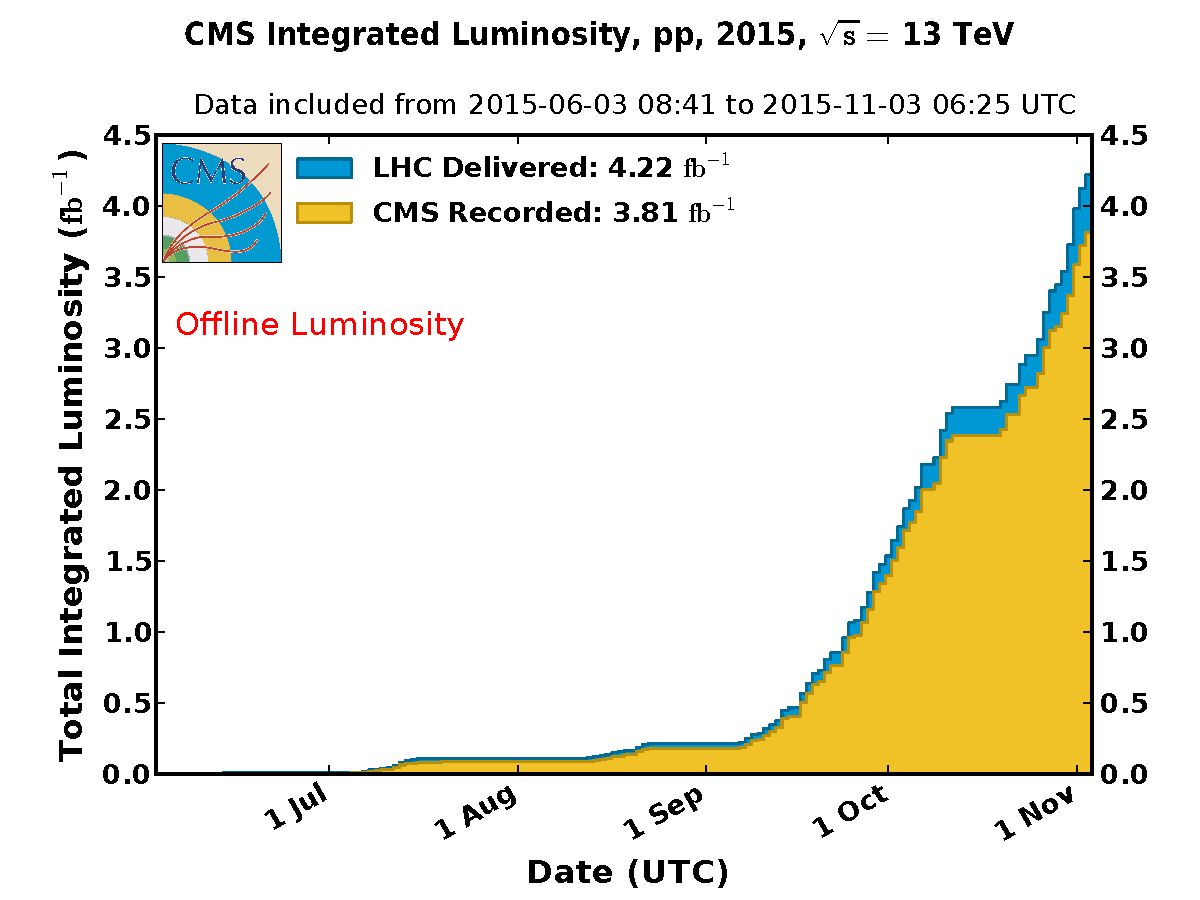
\includegraphics[width=1.0\textwidth]{figures/int_lumi_per_day_cumulative_pp_2015.pdf}
	\caption{Integrated luminosity delivered by the LHC, and recorded by CMS in 2015.}
	\label{fig:lhc2015IntegLumi}
\end{figure}


The raw dataset collected by CMS is too large ($\gtrsim 10^{4}$ terabytes) to process for analyses
which want to run from start to finish in $\lessim 3$ days, and contains much more information
than what is needed by any individual physics analysis.  To expedite the process of
transforming collision data into a public physics result, collision data from each run
era is split into several smaller datasets which are distinguished by the presence of one
or more objects in the final state, such as events with at least one muon, or least two
electrons or photons.  The HLT decides which dataset an event should be assigned to based on the
individual triggers which were fired; in some instances one event will be assigned to several
datasets.  As the average instantaneous luminosity of the LHC increased dramatically in the 
last 3 months of data-taking, datasets in Run2015D were split into two pieces such that the size
of each dataset remained small ($\sim 1$ terabyte).  The collision events used in this analysis
were collected in the "SingleMuon", "DoubleEG", and "MuonEG" datasets summarized in Table
\ref{tab:collisionDatasets}.  This analysis uses the datasets which were reconstructed, the process
by which raw detector outputs are transformed into distinguishable objects like muons and
electrons, in the late summer, fall and early winter of 2015 using calibration and alignment
constants derived in early 2015.

\begin{table}[h]
\caption{The collision datasets used in this analysis, the run eras they correspond to, and their total size (both dataset pieces for 2015D).}
\label{tab:collisionDatasets}
\centering
\begin{tabular}{c|c|c|c|c}
Run Era & Int. Lumi (pb$^{-1}$) & eejj dataset & $\mu\mu$jj dataset & e$\mu$jj dataset \\  \hline
	2015C &  CLUMI  &  DoubleEG  &  SingleMuon  &  MuonEG  \\
	2015D &  DLUMI  &  DoubleEG  &  SingleMuon  &  MuonEG  \\ \hline
\end{tabular}
\end{table}

The "DoubleEG" dataset requires at least two energetic energy deposits in ECAL 
consistent with electrons or photons.  It is used to study events with two electrons and two jets
in the final state, and to look for evidence of \WR bosons which decay to electron flavor
heavy neutrinos.  During collisions, events are selected using the trigger $\verb|HLT_DoubleEle33_CaloIdL_GsfTrkIdVL|$.
As explained in Chapter \ref{sec:experiment_chapter}, the trigger runs a subset of the full
particle reconstruction software package to reconstruct electron candidates in
every event.  After reconstruction, the trigger requires at least two electrons to pass
the cuts defined in Table \ref{tab:eleHltCuts}.  These cuts were optimized to increase the fraction
of real electrons selected relative to the number of fake electrons, coming from QCD and other
sources, selected by the trigger.  The ID variable cut thresholds differ between the ECAL barrel ($|\eta| \leq 1.42$)
and endcap ($|\eta| \geq 1.57$) for the following reason.  All ECAL crystals are used for event
triggering, but the way in which these crystals are grouped into trigger zones differs between the
barrel and endcap.  As a result, the shape and peak position of ID variables for real electrons
produced by $Z \rightarrow ee$ decays differs between barrel and endcap electrons.  The electron
ID variable cut thresholds differ between the barrel and endcap such that each ID cut selects
real barrel and endcap electrons with similar efficiencies.


\begin{table}[h]
\caption{Double electron trigger requirements. NOT COMPLETE FINISH LATER}
\label{tab:eleHltCuts}
\centering
\begin{tabular}{c|c|c}
	Variable & Barrel cut threshold & Endcap cut threshold  \\  \hline
	energy and geometric acceptance cuts  &  &   \\
	$E_{T} (\GeV)$  &  33  &  33  \\
	$|\eta| (-)$  &  $< 2.5$  &  $< 2.5$  \\  \hline
	electron ID cuts  &  &  \\
	$\sigma_{i\eta i\eta} (-)$  &  $< 0.014$  &  $< 0.035$  \\
	$H/E (1/\GeV)$  &  $< 0.15/E_{T}$  &  $< 0.1/E_{T}$  \\
	ECAL Iso $(1/\GeV)$  &  $< EBISO/E_{T}$  &  $< EEISO/E_{T}$  \\
\end{tabular}
\end{table}


This particular double electron trigger was chosen based on trigger efficiency, and offline (post trigger)
requirements which must be tighter than the trigger.  As shown in
Table \ref{tab:singleAndDblEleTriggers}, there is not a significant difference in trigger efficiency
between single and double electron triggers as long as single electron Level 1 triggers are utilized.
These efficiencies were calculated using events from the 800 $\GeV$ \WR mass $\WR \rightarrow eejj$
dataset, as events from this dataset have the lowest average leading and subleading electron $E_{T}$
of all $\WR \rightarrow eejj$ datasets considered in this search.  To allow the offline (post trigger)
electron energy cuts to be as low as possible for increased signal acceptance, and to allow the HEEP
offline electron ID requirements to be used, $\verb|HLT_DoubleEle33_CaloIdL_GsfTrkIdVL|$ was chosen
over the higher $E_{T}$ and tighter ID single electron trigger.

\begin{table}[h]
\caption{Efficiency of electron triggers in 800 $\GeV$ \WR mass $\WR \rightarrow eejj$ signal events which have
two real, reconstructed electrons within the trigger acceptance ($|\eta| \leq 2.5$).  The double electron trigger
with lower $E_{T}$ cuts (23 and 12) can only fire if a double electron Level 1 trigger is fired, and thus has
a lower efficiency than the DoubleEle33 trigger which can fire if a double or single electron Level 1 trigger
is fired.}
\label{tab:singleAndDblEleTriggers}
\centering
\begin{tabular}{c|c|}
	Electron trigger & Efficiency (\%)  \\  \hline
	$\verb|HLT_Ele105_CaloIdVT_GsfTrkIdT|$  &  $94.8\pm0.2$  \\
	$\verb|HLT_DoubleEle33_CaloIdL_GsfTrkIdVL|$  &  $92.0\pm0.2$  \\
	$\verb|HLT_Ele23_Ele12_CaloIdL_TrackIdL_IsoVL|$  &  $91.0\pm0.2$  \\
\end{tabular}
\end{table}

The "SingleMuon" dataset requires.


\subsection{Monte Carlo}
\label{MC}


%%%%%%%%%%%%%%%%%%%%%%%%%%%%%%%%%%%%%%%%%%%%%%%%%%%%%%%%%%%%%%%%%%%%%%%%%%%%%%%%
